\section{Case Studies}
\label{sec:caseStudy}
In order to quantify the effects of optimizing the scripts, we performed a case study.
We say that a C\# method is {\em intrinsicable} if it is a .NET Framework method for which the SCOPE compiler has a semantically equivalent C++ function.
The jobs were chosen based on a static analysis that found {\em optimizable vertices}.
An optimizable vertex is one that is implemented in C\#, but the C\# code calls only intrinsicable methods or user-defined functions, {\em UDFs}, where the UDF, in turn, calls only intrinsicable methods, and does not call any other UDFs, i.e., our inlining depth is one.
We then manually looked at the top jobs from  a ranked list (by CPU time) of jobs containing an optimizable vertex.

Because the input data for each job is not available, we needed to contact the job owners and ask them to re-run the job with a manually-inlined version of their script.
We were able to have only a few jobs re-run by their owners.
We roughly categorize the jobs by their total CPU time: short, medium, and long.

\subsection{Optimizations With Effects On Job Algebra}
As explained in Section~\ref{sec:intro}, the optimizer may choose to modify the job algebra given the new information available to it.
For example, predicates might be pushed deeper into the DAG which can result in dramatic data reduction.
However, none of the case studies ended up causing this kind of optimization.


\subsection{Optimizations Without Effects On Job Algebra}
Even if the physical plan does not change, the resulting program might be might more efficient if it avoids the native to managed transition.
For SCOPE, the set of intrinsics means that by lifting more non-relational code into the parts of the program where such things are visible to the optimizer, more code can be executed in C++ instead of in C\#.

For instance, Job A is a medium-expensive job that runs daily which contains exactly one optimizable vertex due to a UDF.
Inlining that UDF resulted in the entire vertex being executed in C++.
Figure~\ref{fig:CaseStudyA} shows the CPU time for that vertex over an 18 day period, the last 5 of which were with the inlined UDF.
The values are normalized by the average of the unoptimized execution times; the optimized version saves approximately 60\% of the execution time.

\begin{figure}[ht]
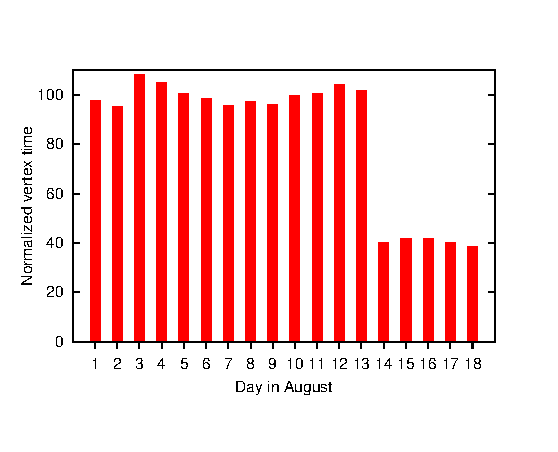
\includegraphics{graphs/normalizedTimes}
\caption{Case Study A \label{fig:CaseStudyA}}
\end{figure}

On the other hand, Job B is similar to Job A: it is also a medium-expensive job which runs daily and contains one optimizable vertex due to a UDF.
However, as Figure~\ref{fig:CaseStudyB} shows, the normalized vertex CPU time does not show any consistent improvement for the last five jobs.
We believe that this is due to the high variability of the job; by all of our measures, CPU time or througput, per vetex or for the full job, Job B displays a wide range of behavior on a daily basis.
\begin{figure}[ht]
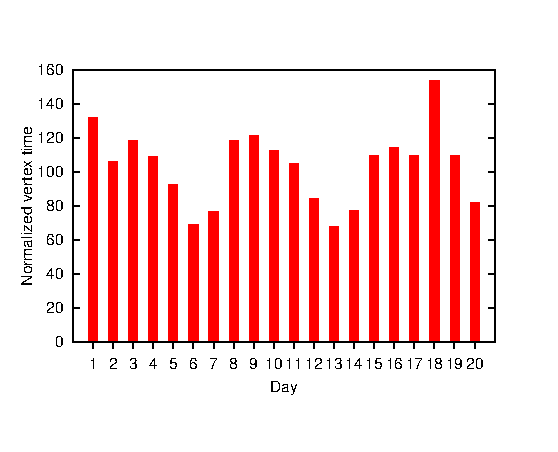
\includegraphics{graphs/normalizedTimesB}
\caption{Case Study B \label{fig:CaseStudyB}}
\end{figure}


We looked at 3 other jobs, summarized in Figure~\ref{fig:caseStudySummary}.
One of them turned out to be a false positive, where we mistakenly thought a method was an intrinsic.
For the other two, we were not able to perform the same kind of historical study: instead we have just one execution of the optimized script.
\begin{figure}[ht]
\begin{tabular}{c|c|c|c|c|c} 
{\em Job Guid} & {\em Vertex} & {\em Job Name} & {\em Job Cost} & {\em Vertex Improvement} & {\em Job Improvement} \\ \hline
01e72a39 & SV4\_Extract & C & low & 41.98\% & 25.00\% \\
0414cd51 & & D & false positive \\
f2bd0961 & SV1\_Extract\_Combine\_Split & E & high & 7.22\% & 4.79\%
\end{tabular}
\caption{Summary of case studies. {\sc Delete the job guid and vertex columns before submitting!}
\label{fig:caseStudySummary}}
\end{figure}

